\section{Additional Results and Simulations for Logarithmic Power-Law Spectrum}\label{app:log-spectrum}
\subsection{Scaling Law for Logarithmic Power-Law Spectrum}
We now present the scaling law for a logarithmic power-law spectrum.
% \kaifengclaw{Style: consider 'a logarithmic power-law spectrum' for grammar.} 
Its proof can be seen in \Cref{sec:proof-one-hot-scaling-law-log-spectrum}.
\begin{theorem} \label{thm:one-hot-log-scaling-law}
    Consider a $K$-epoch SGD over $N$ fresh data. Under Assumptions~\ref{asp:parameter-prior}, \Cref{asp:log-power-decay-prior}, and given the data dimension $d = \Omega((KN)^{\frac{1}{a}})$, it holds that
    \[
    \Bar{\cR}^*(K,N) \asymp 
    \begin{cases}
         \left(KN\right)^{-\frac{a-1}{a}} & \text{for } K = o(\log^b N) \\
         {\left(N\log^b N\right)^{-\frac{a-1}{a}}}& \text{for } K = \omega(\log^b N).
    \end{cases}
    \]
\end{theorem}

\subsection{Simulations in \Cref{sec:log-power-spectrum}}

Now we focus on validating the predictions of \Cref{thm:one-hot-E_K-log-spectrum} using synthetic data generated under the spectral assumptions of \Cref{sec:one_hot} and a log-power decay spectrum (\Cref{asp:log-power-decay-prior}).
% Because \Cref{thm:one-hot-loss-estimate} provides a closed-form expression for the multi-epoch loss in these settings, we can perform a more controlled simulation of $E(K,N)$. In particular, we consider two cases: (i) a power-law decay Hessian spectrum (\Cref{asp:prior-probability-and-norm}), and (ii) a log-power decay spectrum (\Cref{asp:log-power-decay-prior}), corresponding to the conditions of \Cref{thm:one-hot-E_K-v2} and \Cref{thm:one-hot-E_K-log-spectrum}, respectively.

\paragraph{Experiments Setup.} Similar to \Cref{sec:power-spectrum-experiment}, in all sub-figures of \Cref{fig:one-hot-log}, we set the data dimension $d$ to $10^5$ and tune all the learning rates to their optimal values. Here we set $a=1.5$ and $b=2$. 
% In the simulations of the power spectrum case, we 
% \paragraph{Simulations in Power Spectrum Case.} 
% The top-left panel of \Cref{fig:one-hot-log} plots $E(K,N)$ versus $\log K$ for various fixed $N$, while the right panels show $E(K,N)$ versus $\log N$ for various fixed $K$. In the power-law spectrum scenario, we observe an initial regime where $E(K,N)$ increases almost linearly with $K$ (indicating that more epochs initially provide almost proportional gains in effective data usage), followed by a clear saturation regime where $E(K,N)$ approaches a constant plateau even as $K$ continues to grow. This plateau value is much lower than $K$ when $K$ is large, and it depends on $N$ in a manner consistent with our theory. Specifically, $E(K,N)$ eventually saturates at an asymptotic value, and larger datasets yield higher saturation levels, reflecting a dataset-dependent multiple-epoch benefit, as predicted by \Cref{thm:one-hot-E_K-v2}.  

% % \begin{figure}[htbp]
% % \begin{figure}[t!]
% %     \centering
% %     \includegraphics[width=0.6\linewidth]{figures/one-hot-simulation/E_K_comparison_2x2_paper.pdf}
% %     \caption{Simulation results in the solvable case with power law. \textbf{Top-Left:}}
% %     \label{fig:one-hot-log}
% % \end{figure}

% \paragraph{Simulations in Log-Power Spectrum Case.} 
% In the log-power spectrum setting (bottom panels of \Cref{fig:one-hot-log}), $E(K,N)$ exhibits a similar two-regime behavior: the initial growth with $K$ transitions to a plateau whose height increases only logarithmically with $N$ (on the order of $\log^b N$), as described by \Cref{thm:one-hot-E_K-log-spectrum}. The curves depicting $E(K,N)$ versus $\log N$ further illustrate that, for fixed small values of $K$, increasing $N$ eventually yields diminishing returns as $E(K,N)$ approaches the $K$ limit (analogous to the strongly-convex case). For larger values of $K$, however, the effective multiplier reaches a ceiling determined by the dataset-dependent saturation value. These experiments demonstrate the anticipated saturation effects, multiple scaling regimes, and asymptotic plateaus, providing empirical confirmation of the scaling behaviors predicted by \Cref{thm:one-hot-E_K-v2} and \Cref{thm:one-hot-E_K-log-spectrum}.




\paragraph{Simulations for the Solvable Model.} \Cref{fig:one-hot-log} plots $E(K, N)$ versus $K$ and $\log N$ for the solvable model. The curves depicting $E(K,N)$ versus $K$ and $E(K,N)$ versus $\log N$ show trends consistent with those in \Cref{sec:power-spectrum-experiment}, aligning with \Cref{thm:one-hot-E_K-log-spectrum}. 
% The top line and the bottom line show the plots in power spectrum case and log-power spectrum case respectively. For both cases, the curves depicting $E(K,N)$ versus $K$ show that $E(K,N)\approx K$ when $K$ is relatively small and saturate to some value depending on $N$ when $K$ is large. In the right panels, which describe the relationship between $E(K,N)$ and $\log N$, we observe that when $K$ is small (namely $K=2$), $E(K,N)$ increases and approaches $K$ as $\log N$ increases, and the plots overlap when $K$ is large. Those pheomena provide empirical confirmation of the scaling behaviors predicted by \Cref{thm:one-hot-E_K-v2} and \Cref{thm:one-hot-E_K-log-spectrum}. 
Furthermore, in the large-$K$ regime, we fit the exponent according to \Cref{thm:one-hot-E_K-log-spectrum} and obtain $2.036 \approx b = 2$, which provides strong validation of our theory.


% We now verify the predictions of \Cref{thm:one-hot-E_K-v2} and \Cref{thm:one-hot-E_K-log-spectrum} using synthetic data generated under the spectral assumptions of \Cref{sec:one_hot}. Because \Cref{thm:one-hot-loss-estimate} provides a closed-form expression for the multi-epoch loss in these settings, we can perform a more controlled simulation of $E(K,N)$. In particular, we consider two cases: (i) a power-law decay Hessian spectrum (\Cref{asp:prior-probability-and-norm}), and (ii) a log-power decay spectrum (\Cref{asp:log-power-decay-prior}), corresponding to the conditions of \Cref{thm:one-hot-E_K-v2} and \Cref{thm:one-hot-E_K-log-spectrum}, respectively.

% \paragraph{Experiments Setup.} In all sub-figures of \Cref{fig:one-hot-log}, we set the data dimension $d$ to $10^5$ and tune all the learning rates to their optimal values. Additionally, we separately tune the spectrum parameters $a$ and $b$ in each sub-figure of \Cref{fig:one-hot-log}. Specifically, in the top-left and top-right panels, we set $a=4.5$ and $b=1$, whereas in the bottom-left and bottom-right panels, we set $a=1.5$ and $b=2$. 
% % In the simulations of the power spectrum case, we 
% % \paragraph{Simulations in Power Spectrum Case.} 
% % The top-left panel of \Cref{fig:one-hot-log} plots $E(K,N)$ versus $\log K$ for various fixed $N$, while the right panels show $E(K,N)$ versus $\log N$ for various fixed $K$. In the power-law spectrum scenario, we observe an initial regime where $E(K,N)$ increases almost linearly with $K$ (indicating that more epochs initially provide almost proportional gains in effective data usage), followed by a clear saturation regime where $E(K,N)$ approaches a constant plateau even as $K$ continues to grow. This plateau value is much lower than $K$ when $K$ is large, and it depends on $N$ in a manner consistent with our theory. Specifically, $E(K,N)$ eventually saturates at an asymptotic value, and larger datasets yield higher saturation levels, reflecting a dataset-dependent multiple-epoch benefit, as predicted by \Cref{thm:one-hot-E_K-v2}.  

% % % \begin{figure}[htbp]
% % % \begin{figure}[t!]
% % %     \centering
% % %     \includegraphics[width=0.6\linewidth]{figures/one-hot-simulation/E_K_comparison_2x2_paper.pdf}
% % %     \caption{Simulation results in the solvable case with power law. \textbf{Top-Left:}}
% % %     \label{fig:one-hot-log}
% % % \end{figure}

% % \paragraph{Simulations in Log-Power Spectrum Case.} 
% % In the log-power spectrum setting (bottom panels of \Cref{fig:one-hot-log}), $E(K,N)$ exhibits a similar two-regime behavior: the initial growth with $K$ transitions to a plateau whose height increases only logarithmically with $N$ (on the order of $\log^b N$), as described by \Cref{thm:one-hot-E_K-log-spectrum}. The curves depicting $E(K,N)$ versus $\log N$ further illustrate that, for fixed small values of $K$, increasing $N$ eventually yields diminishing returns as $E(K,N)$ approaches the $K$ limit (analogous to the strongly-convex case). For larger values of $K$, however, the effective multiplier reaches a ceiling determined by the dataset-dependent saturation value. These experiments demonstrate the anticipated saturation effects, multiple scaling regimes, and asymptotic plateaus, providing empirical confirmation of the scaling behaviors predicted by \Cref{thm:one-hot-E_K-v2} and \Cref{thm:one-hot-E_K-log-spectrum}.

% \paragraph{Simulations for the Solvable Model.} \Cref{fig:one-hot-log} plots $E(K, N)$ versus $K$ and $\log N$ for the solvable model. The top line and the bottom line show the plots in power spectrum case and log-power spectrum case respectively. For both cases, the curves depicting $E(K,N)$ versus $K$ show that $E(K,N)\approx K$ when $K$ is relatively small and saturate to some value depending on $N$ when $K$ is large. In the right panels, which describe the relationship between $E(K,N)$ and $\log N$, we observe that when $K$ is small (namely $K=2$), $E(K,N)$ increases and approaches $K$ as $\log N$ increases, and the plots overlap when $K$ is large. Those pheomena provide empirical confirmation of the scaling behaviors predicted by \Cref{thm:one-hot-E_K-v2} and \Cref{thm:one-hot-E_K-log-spectrum}. We also fit exponents base on \Cref{thm:one-hot-E_K-v2} and \Cref{thm:one-hot-E_K-log-spectrum} in large-$K$ regime. In the power-spectrum case, the fitted exponent is $0.279 \approx \tfrac{b}{a-b} = \tfrac{2}{7}$, while in the log-spectrum case, the fitted exponent is $2.036 \approx b = 2$, perfectly validating our theory.


% We now verify the predictions of \Cref{thm:one-hot-E_K-log-spectrum} using synthetic data generated under the spectral assumptions of \Cref{sec:one_hot} 
% % Because \Cref{thm:one-hot-loss-estimate} provides a closed-form expression for the multi-epoch loss in these settings, we can perform a more controlled simulation of $E(K,N)$. 
% % In particular, we consider two cases: (i) 
% with a power-law decay Hessian spectrum (\Cref{asp:prior-probability-and-norm}).


% % We now verify the predictions of \Cref{thm:one-hot-E_K-log-spectrum} using synthetic data generated under the spectral assumptions of \Cref{sec:one_hot} 
% % % Because \Cref{thm:one-hot-loss-estimate} provides a closed-form expression for the multi-epoch loss in these settings, we can perform a more controlled simulation of $E(K,N)$. 
% % % In particular, we consider two cases: (i) 
% % with a power-law decay Hessian spectrum (\Cref{asp:prior-probability-and-norm}).

% % % , and (ii) a log-power decay spectrum (\Cref{asp:log-power-decay-prior}), corresponding to the conditions of \Cref{thm:one-hot-E_K-v2} and \Cref{thm:one-hot-E_K-log-spectrum}, respectively.

% % \paragraph{Experiments Setup.} In all sub-figures of \Cref{fig:one-hot-log}, we set the data dimension $d$ to $10^5$ and tune all the learning rates to their optimal values. Here we set $a=1.5$ and $b=2$. 

% % % . Additionally, we separately tune the spectrum parameters $a$ and $b$ in each sub-figure of \Cref{fig:one-hot-log}. Specifically, in the top-left and top-right panels, we set $a=4.5$ and $b=1$, whereas in the bottom-left and bottom-right panels, we set $a=1.5$ and $b=2$. 
% % % In the simulations of the power spectrum case, we 
% % % \paragraph{Simulations in Power Spectrum Case.} 
% % % The top-left panel of \Cref{fig:one-hot-log} plots $E(K,N)$ versus $\log K$ for various fixed $N$, while the right panels show $E(K,N)$ versus $\log N$ for various fixed $K$. In the power-law spectrum scenario, we observe an initial regime where $E(K,N)$ increases almost linearly with $K$ (indicating that more epochs initially provide almost proportional gains in effective data usage), followed by a clear saturation regime where $E(K,N)$ approaches a constant plateau even as $K$ continues to grow. This plateau value is much lower than $K$ when $K$ is large, and it depends on $N$ in a manner consistent with our theory. Specifically, $E(K,N)$ eventually saturates at an asymptotic value, and larger datasets yield higher saturation levels, reflecting a dataset-dependent multiple-epoch benefit, as predicted by \Cref{thm:one-hot-E_K-v2}.  

% % % % \begin{figure}[htbp]
% % % % \begin{figure}[t!]
% % % %     \centering
% % % %     \includegraphics[width=0.6\linewidth]{figures/one-hot-simulation/E_K_comparison_2x2_paper.pdf}
% % % %     \caption{Simulation results in the solvable case with power law. \textbf{Top-Left:}}
% % % %     \label{fig:one-hot-log}
% % % % \end{figure}

% % % \paragraph{Simulations in Log-Power Spectrum Case.} 
% % % In the log-power spectrum setting (bottom panels of \Cref{fig:one-hot-log}), $E(K,N)$ exhibits a similar two-regime behavior: the initial growth with $K$ transitions to a plateau whose height increases only logarithmically with $N$ (on the order of $\log^b N$), as described by \Cref{thm:one-hot-E_K-log-spectrum}. The curves depicting $E(K,N)$ versus $\log N$ further illustrate that, for fixed small values of $K$, increasing $N$ eventually yields diminishing returns as $E(K,N)$ approaches the $K$ limit (analogous to the strongly-convex case). For larger values of $K$, however, the effective multiplier reaches a ceiling determined by the dataset-dependent saturation value. These experiments demonstrate the anticipated saturation effects, multiple scaling regimes, and asymptotic plateaus, providing empirical confirmation of the scaling behaviors predicted by \Cref{thm:one-hot-E_K-v2} and \Cref{thm:one-hot-E_K-log-spectrum}.

% % \paragraph{Simulations for the Solvable Model.} \Cref{fig:one-hot-log} plots $E(K, N)$ versus $K$ and $\log N$ for the solvable model. The curves depicting $E(K,N)$ versus $K$ show that $E(K,N)\approx K$ when $K$ is relatively small and saturate to some value depending on $N$ when $K$ is large. In the right panel, which describe the relationship between $E(K,N)$ and $\log N$, we observe that when $K$ is small (namely $K=2$), $E(K,N)$ increases and approaches $K$ as $\log N$ increases, and the plots overlap when $K$ is large. Those pheomena provide empirical confirmation of the scaling behaviors predicted by \Cref{thm:one-hot-E_K-v2}. We also fit exponents based on \Cref{thm:one-hot-E_K-v2} in the large-$K$ regime. In the power-spectrum case, the fitted exponent is $0.279 \approx \tfrac{b}{a-b} = \tfrac{2}{7}$, perfectly validating our theory.
% % % \vspace{-0.4mm}
% We now verify the predictions of \Cref{thm:one-hot-E_K-v2} and \Cref{thm:one-hot-E_K-log-spectrum} using synthetic data generated under the spectral assumptions of \Cref{sec:one_hot}. Because \Cref{thm:one-hot-loss-estimate} provides a closed-form expression for the multi-epoch loss in these settings, we can perform a more controlled simulation of $E(K,N)$. In particular, we consider two cases: (i) a power-law decay Hessian spectrum (\Cref{asp:prior-probability-and-norm}), and (ii) a log-power decay spectrum (\Cref{asp:log-power-decay-prior}), corresponding to the conditions of \Cref{thm:one-hot-E_K-v2} and \Cref{thm:one-hot-E_K-log-spectrum}, respectively.
\begin{figure}[t!]
    % \vspace{-0.7in}
    \centering
    % \begin{subfigure}[b]{0.98\linewidth} 
    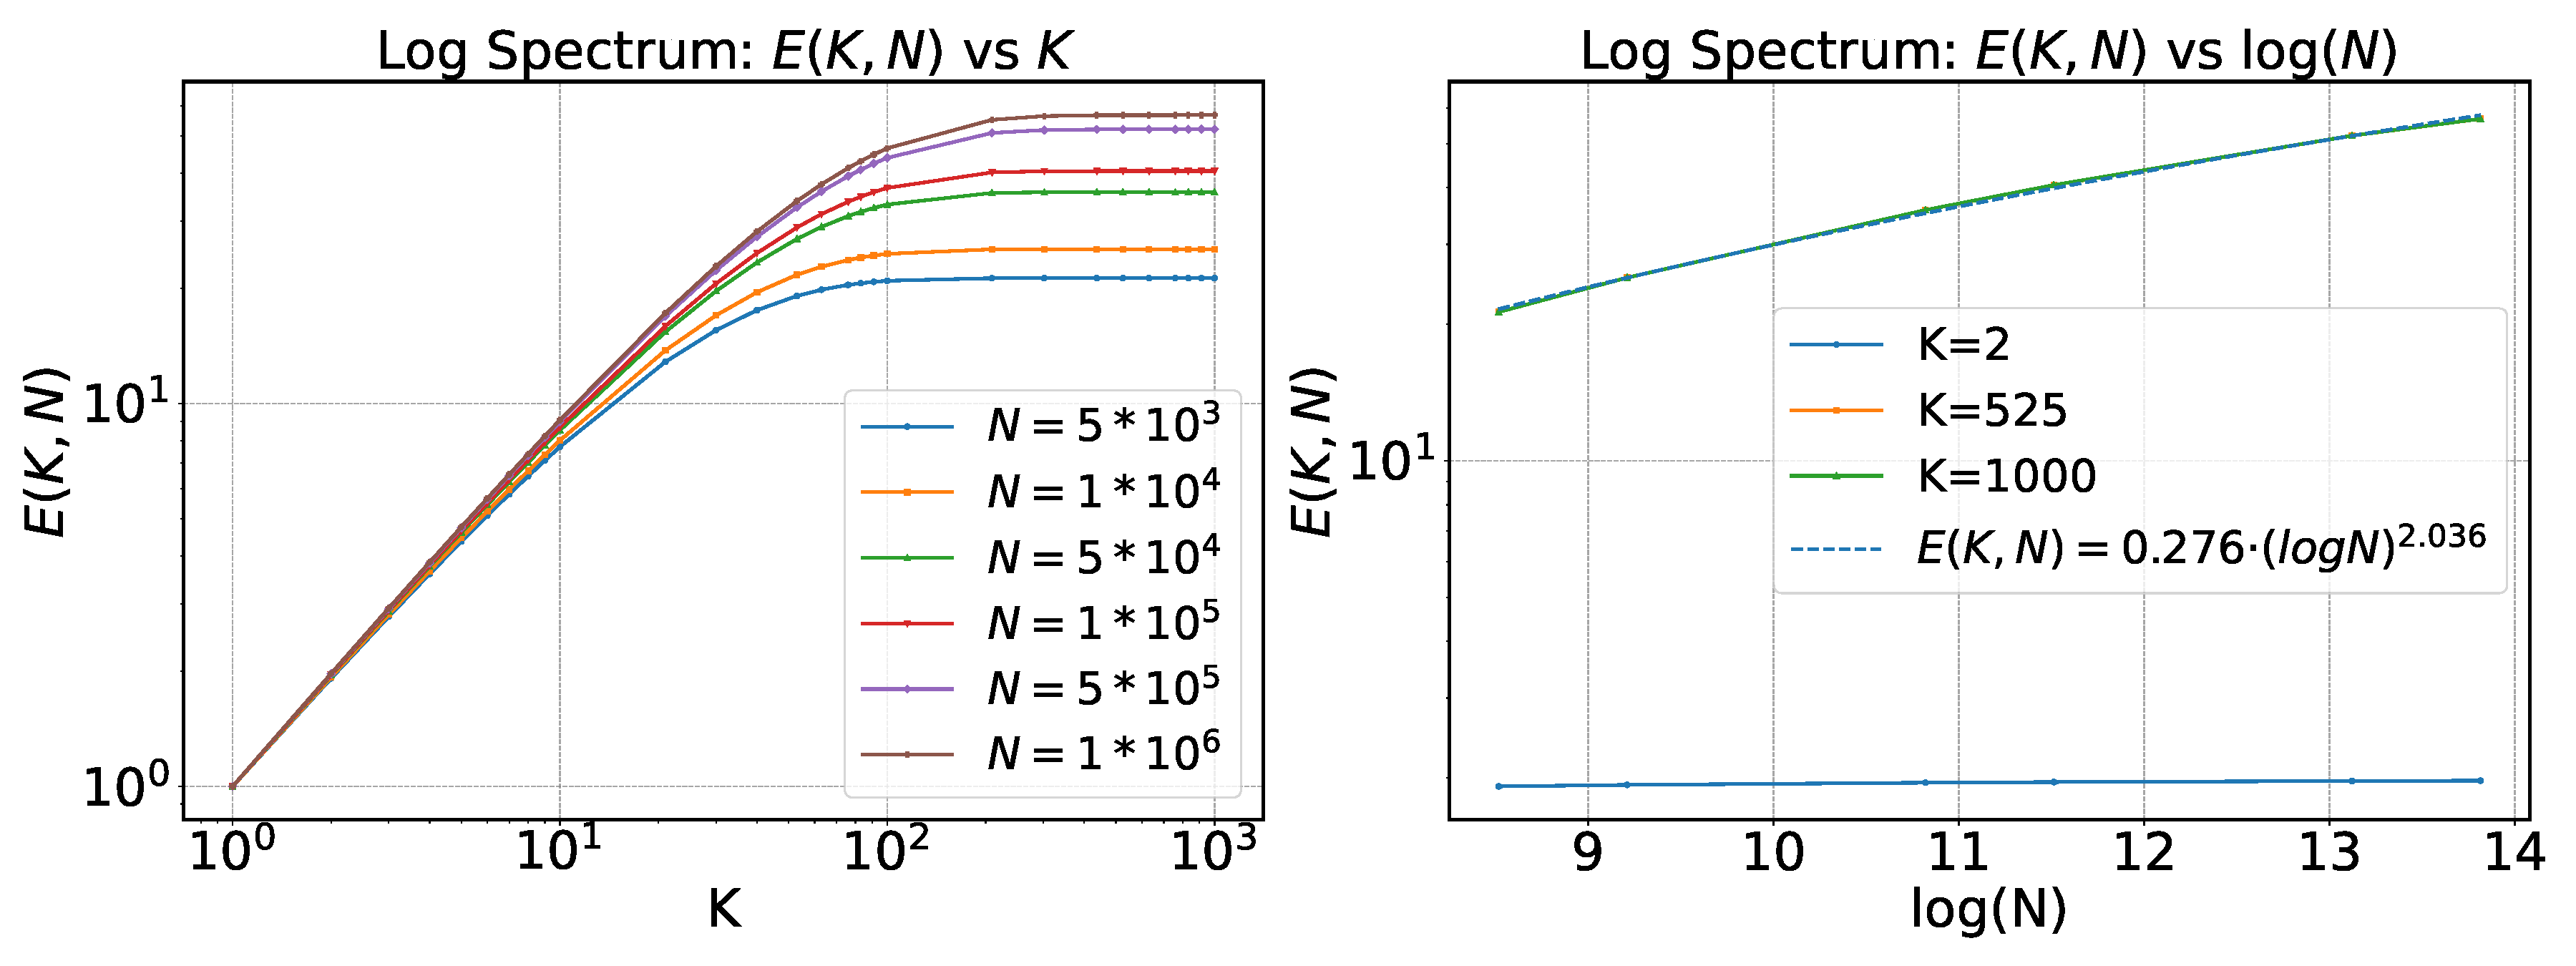
\includegraphics[width=\linewidth]{figs/E_K_comparison_log.pdf}
         \caption{The solvable cases with logarithmic power-law spectrum. $E(K,N)$ exhibits a similar behavior to that presented in \Cref{fig:convex-and-power}. We also fit the effective reuse rate using the formula $E(K,N)=c_1\left(\log N\right)^{c_2}$ suggested by \Cref{thm:one-hot-E_K-log-spectrum}, and the fitted exponent $c_2=2\approx b=2$ matches our theory.}
         % \kaifengclaw{Reference logic: this log-spectrum fit is more directly tied to \Cref{thm:one-hot-E_K-log-spectrum}; consider citing that theorem here.}
        % \caption{The effective reuse rate $E(K,N)$ as a function of the number of training epochs $K$ for varying fresh data sizes $N$. The shaded regions represent the variability from the smoothed trend in different epochs.}
        \label{fig:one-hot-log}
    % \end{subfigure}   
\end{figure}